%%%%%%%%%%
% TESTING PAUSE DETECTION
%%%%%%%%%%
\subsection{Test 1: Testing Pause Detection}
\subsubsection{\underline{Test 1.1: Four controlled pauses}}
\begin{description}
	\item[Test:] The test aimed to see at what level calpy could identify each pause. 
				An utterance was recorded by the author and copied three times to produce four pauses in total.
				The pauses were 1s, 10ms, 1ms and 3s respectively.
				The 1ms pause is marked by the black line in the soundwave, otherwise it's too small to be seen.
	\item[File:] The file used was data/pause\_test/500ms\_40ms\_1ms\_3s/ \\
	\space\space\space\space 44100/500ms\_40ms\_1ms\_3s\_44100.wav
	\item[Result:] 3 out of 4 pauses were accounted for. The 1ms pause was not detected.
\end{description}
\begin{figure}[h]
	\center
	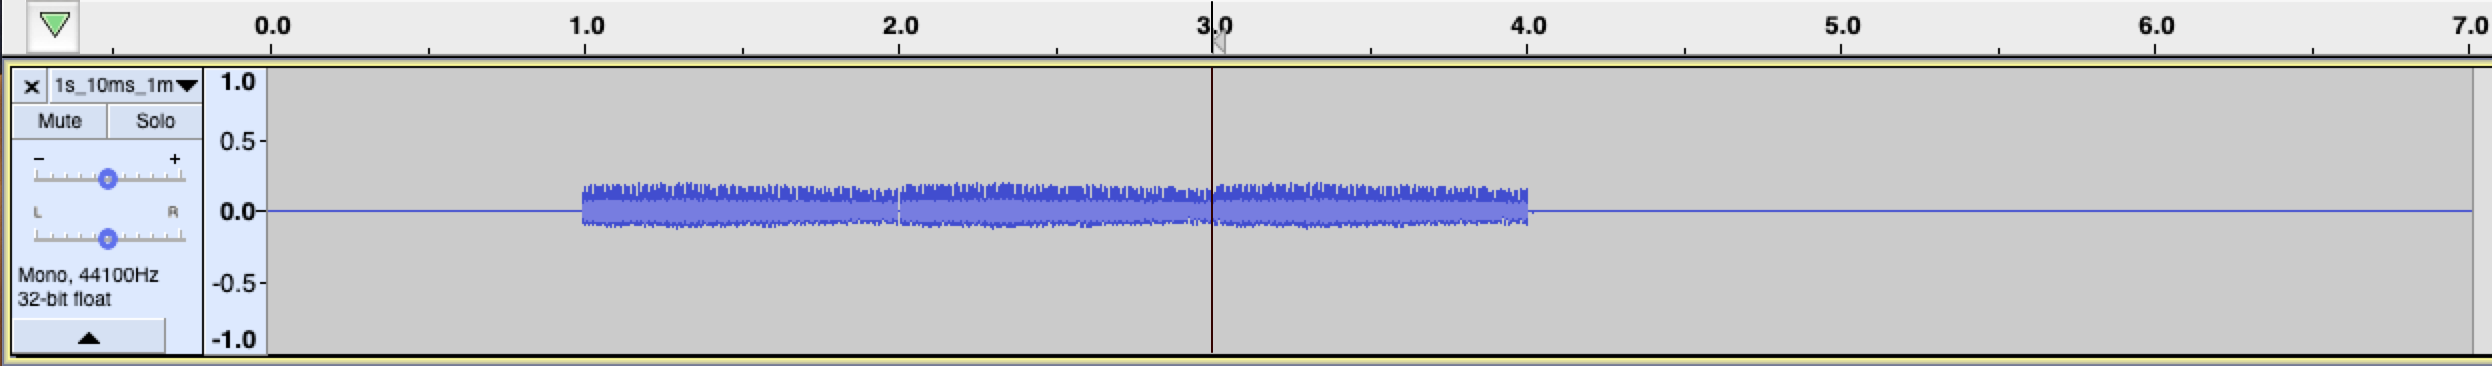
\includegraphics[scale=0.3]{src/main-matter/results/preliminary-testing/detection/1s_10ms_1ms_3s}
	\caption{Waveform of Test 1.1}
	\label{fig:011}
\end{figure}

\subsubsection{\underline{Test 1.2: Counting one to eight}}
\begin{description}
	\item[Test:] The numbers one to eight were counted by the author (very slowly with ample pause) to see where pauses are and aren't detected.
	\item[File:] The file used was data/pause\_test/detection/counting/one\_to\_eight\_robert.wav and can be found in the accompanying data source provided.
	\item[Result:] 9 pauses were accounted for out of a total 9. 
\end{description}
\begin{figure}[h]
	\center
	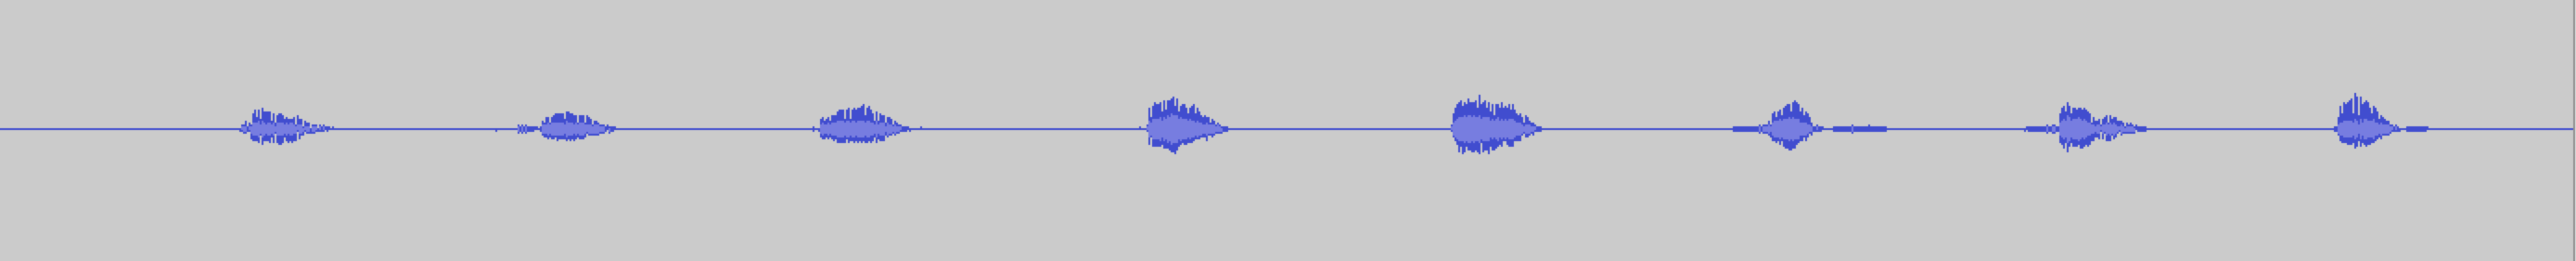
\includegraphics[scale=0.2]{src/main-matter/results/preliminary-testing/detection/011}
	\caption{Waveform of Test 1.2}
	\label{fig:011}
\end{figure}
%
%\paragraph{\underline{Test 1.3: Counting one - Extending initial pause}}
%\begin{description}
%	\item[\underline{Test:}] Seeing where the pause from Test 1.1 is being left out. The audio file from Test 1.1 was taken 
%						and cut down to just the first utterance and surrounding pauses. The initial pause was extended 
%						to help differentiate between the potential returned lengths
%	\item[\underline{File:}] data/pause\_test/detection/counting/one\_robert.wav 
%	\item[\underline{Result:}] A single pause of length 6 was returned
%\end{description}
%\begin{figure}[h]
%	\center
%	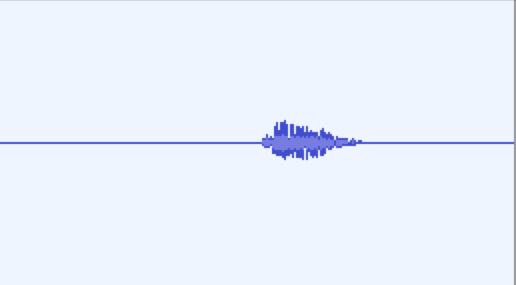
\includegraphics[scale=0.2]{src/main-matter/results/preliminary-testing/detection/012}
%	\caption{}
%	\label{fig:012}
%\end{figure}


%\paragraph{\underline{Test 1.3: Counting one - Extending final pause}}
%\begin{description}
%	\item[\underline{Test:}] The audio from Test 1.2 was used with the final pause extended out
%	\item[\underline{File:}] data/pause\_test/detection/counting/one\_long\_end\_padding\_robert.wav
%	\item[\underline{Result:}] A single pause of length 6 was returned 
%\end{description}
%\begin{figure}[h]
%	\center
%	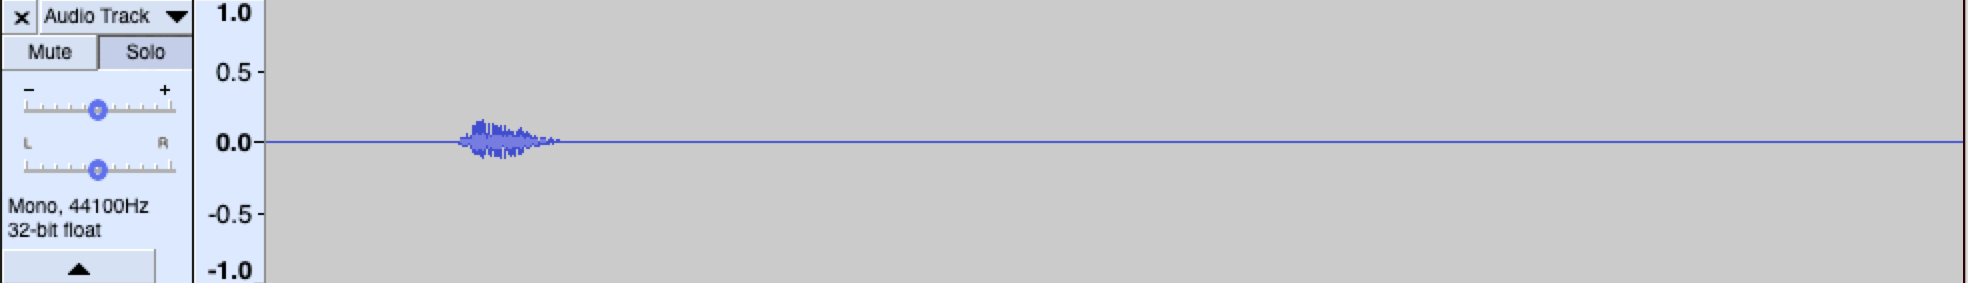
\includegraphics[scale=0.2]{src/main-matter/results/preliminary-testing/detection/013}
%	\caption{}
%	\label{fig:013}
%\end{figure}


%\paragraph{\underline{Test 1.4: Counting one - Further extending initial pause}}
%\begin{description}
%	\item[\underline{Test:}] The audio from Test 1.2 was used with the initial pause further extended to confirm 
%						only the last pause isn't detected
%	\item[\underline{File:}] data/pause\_test/detection/counting/one\_long\_start\_padding\_robert.wav
%	\item[\underline{Result:}] A pause of length 20 was returned 
%\end{description}
%\begin{figure}[h]
%	\center
%	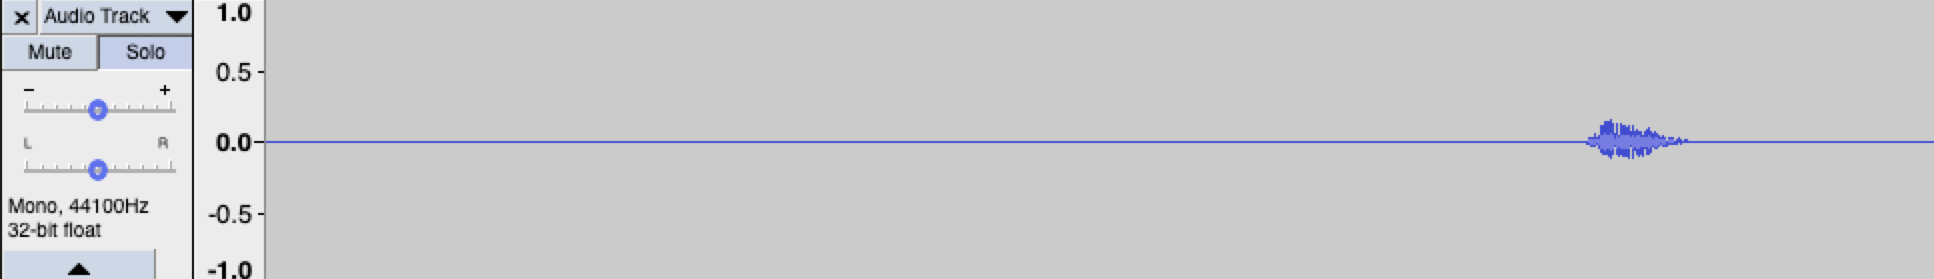
\includegraphics[scale=0.2]{src/main-matter/results/preliminary-testing/detection/014}
%	\caption{}
%	\label{fig:014}
%\end{figure}

\paragraph{\underline{Test 1.3: Counting one to four - Background noise}}
\begin{description}
	\item[Test:] A new audio file was made of the author counting one to four 
				with low background noise of a fan included during recording 
	\item[File:] data/pause\_test/detection/counting/one\_to\_four\_bkg\_fan\_robert.wav
	\item[Result:] 5 pauses returned out of a total 5
\end{description}
\begin{figure}[h]
	\center
	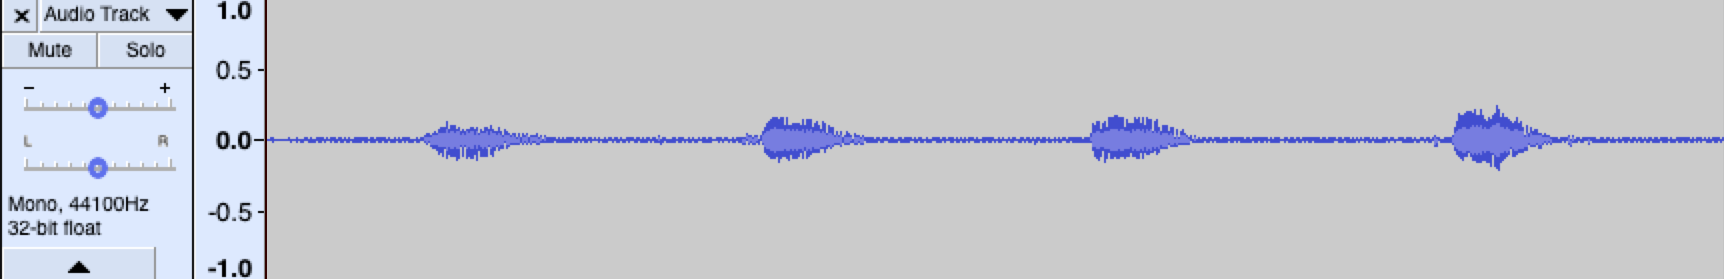
\includegraphics[scale=0.2]{src/main-matter/results/preliminary-testing/detection/015}
	\caption{Waveform of Test 1.3}
	\label{fig:015}
\end{figure}

\paragraph{\underline{Test 1.4: Counting one to five - Background Noise}}
\begin{description}
	\item[Test:] A similar test to test 1.5 with higher intensity background noise 
	\item[File:] data/pause\_test/detection/counting/one\_to\_five\_bkg\_fan\_robert.wav
	\item[Result:] 6 pauses returned out of a total 6
\end{description}
\begin{figure}[h]
	\center
	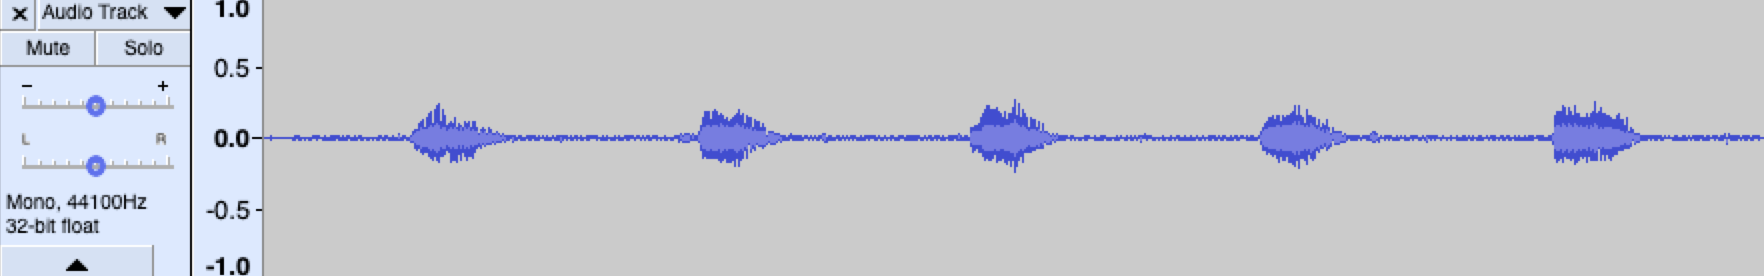
\includegraphics[scale=0.2]{src/main-matter/results/preliminary-testing/detection/016}
	\caption{Waveform of Test 1.4}
	\label{fig:016}
\end{figure}

\paragraph{\underline{Test 1.5: Counting one to six - Relaxed delivery}}
\begin{description}
	\item[Test:] Author counted one to six in a more relaxed speech delivery 
	\item[File:] data/pause\_test/detection/counting/one\_to\_six\_relaxed.wav
	\item[Result:] 7 out of 7 pauses detected. %No pause was detected between the fifth and sixth utterance
\end{description}
\begin{figure}[h]
	\center
	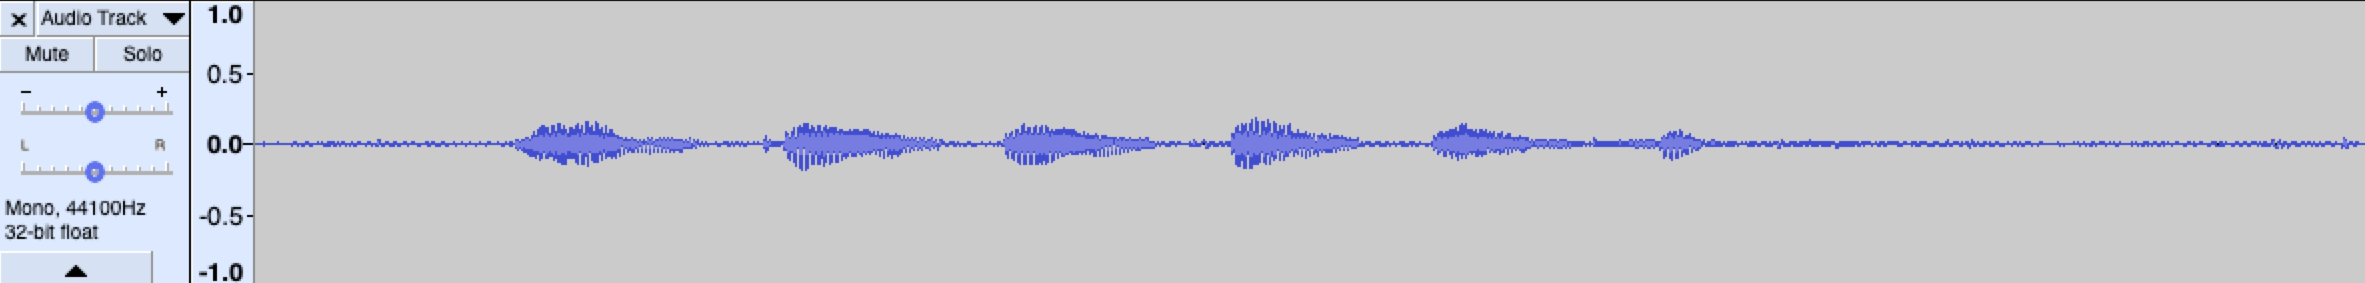
\includegraphics[scale=0.2]{src/main-matter/results/preliminary-testing/detection/017}
	\caption{Waveform of Test 1.5}
	\label{fig:017}
\end{figure}


%\paragraph{\underline{Test 1.8 - Testing Pause Detection - Prose}}
%\begin{description}
%	\item[\underline{Test:}] Author tested in a less controlled speech example by
%						reading a novel for 7 seconds with background noise.  
%	\item[\underline{File:}] data/pause\_test/detection/prose/catch22\_pg1\_7sec.wav
% 	\item[\underline{Output:}]
%	\item[\underline{Result:}] 7 pauses detected out of a total 11 that were intended. 
%%						Of the 9, 2 were pauses less than 1 ms. 
%						Wave form is less distinct as to where pauses are in the audio and shows a 
%						much smoother rise and fall. 
%%						Already this shows a potential breakdown in pause detection. 
%						Results: From the experiment shows micro pause detection doesn't affect the outcome. 
%						This is important because we are not only looking for higher level pauses but also pauses 
%						between words and sentences. 
%\end{description}
%\begin{figure}[h]
%	\center
%	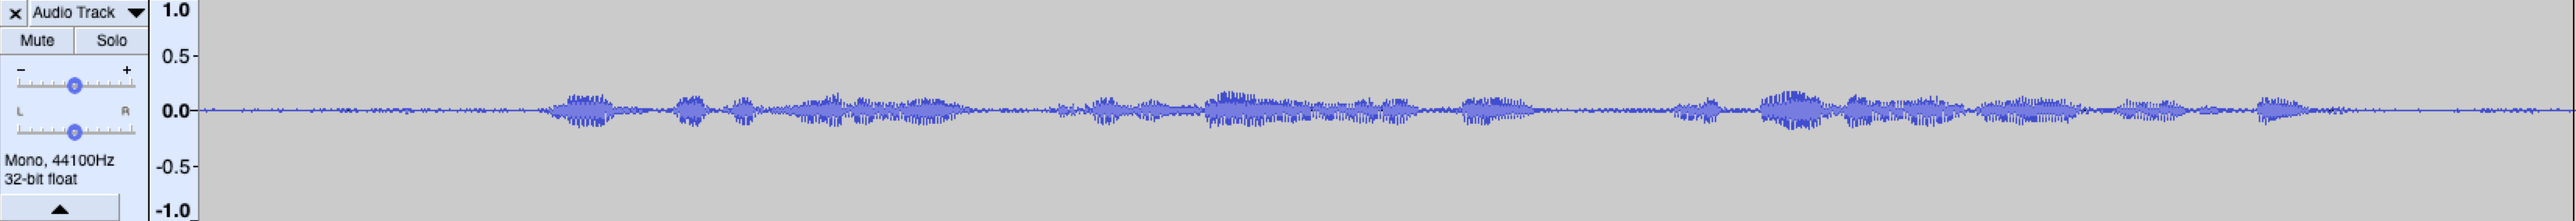
\includegraphics[scale=0.2]{src/main-matter/results/preliminary-testing/detection/018}
%	\caption{}
%	\label{fig:018}
%\end{figure}
